\documentclass[11pt]{article}
\usepackage[margin=2.2cm]{geometry}
\usepackage[T1]{fontenc}
\usepackage{lmodern}
\usepackage{amsmath,amssymb}
\usepackage{booktabs}
\usepackage{graphicx}
\usepackage{xcolor}
\usepackage[hidelinks]{hyperref}
\usepackage{array}
\usepackage{caption}
\captionsetup{font=small,labelfont=bf}
\setlength{\parskip}{0.4em}
\setlength{\parindent}{0pt}

\newcommand{\cstar}{c^{*}}
\newcommand{\dmin}{d_{\min}}

\title{A presynaptic eCB-LTD arm for the Chindemi plasticity rule\\[0.3em]
\large Companion note for the V5 arm (GluSynapse v2, L5$\to$L5)}
\author{Dhuruva Priyan Gowri Mariyappan}
\date{4 October 2026}

\begin{document}
\maketitle

\begin{abstract}
The Chindemi calcium rule $\rho(\cstar)$ gives no LTD for L5$\to$L5 pairings at low frequency: 0.1\,Hz,
$\Delta t=-10$\,ms gives 1.01 against 0.69 in the data. At these synapses, timing-dependent LTD is presynaptic and
needs endocannabinoids (eCB). We add one eCB arm to the unchanged postsynaptic rule. Each piece of the arm comes from
a measurement. Postsynaptic Ca$^{2+}$ builds a slowly decaying eCB trace, and the synapse reads it out at its own
presynaptic spike. When the trace is above threshold, release probability steps down towards a measured floor. Two
order rules apply: glutamate that arrives first stops the trace from being primed, and a spine Ca$^{2+}$ rise just
after the pre spike cancels that readout. With the Chindemi parameters left at their earlier values (no refit), the arm
raises the core-target class match from 11/17 to 13/17 and lowers the core $\chi^2$ from 203 to 46.
\end{abstract}

%=====================================================================
\section{Why an extra arm}
In $\rho$, the plasticity outcome is set by the slow calcium variable $\cstar$, a low-pass filter of spine
Ca$^{2+}$ with $\tau=278$\,ms. At L5$\to$L5 synapses, three observations do not fit a rule that only reads $\cstar$:
\begin{enumerate}
  \item Pre-before-post and post-before-pre pairings at 0.1\,Hz bring in almost the same amount of Ca$^{2+}$. Their
        effects are opposite: the $\Delta t=+10$\,ms pairing gives 0.97 and the $\Delta t=-10$\,ms pairing gives 0.69
        (Sj\"ostr\"om et al.\ 2001). The amount of Ca$^{2+}$ alone does not encode spike order.
  \item The LTD needs eCB/CB1 signalling and presynaptic NR2B-containing NMDA receptors
        (Sj\"ostr\"om et al.\ 2003). It is expressed as a lower release probability. In our readout it therefore
        changes $U_{SE}$, not the postsynaptic weight.
  \item The 278\,ms filter is too slow to resolve the order of spikes within a 10--50\,Hz train.
\end{enumerate}
Without the arm, the rule is the reference model CH0: Chindemi $\rho$ with the shaft-Ca$^{2+}$ licence and the NO arm
from the current fit. CH0 gets every low-frequency $-10$\,ms row wrong (Table~\ref{tab:rows}).

%=====================================================================
\section{Biology the arm follows}
\begin{center}
\small
\begin{tabular}{>{\raggedright}p{0.44\linewidth} >{\raggedright\arraybackslash}p{0.48\linewidth}}
\toprule
Observation & Model element \\
\midrule
Postsynaptic Ca$^{2+}$ makes eCB. The sensor sees volume-averaged total Ca$^{2+}$: EGTA and BAPTA block it alike
(Nevian \& Sakmann 2006). A postsynaptic spike is not required (Sj\"ostr\"om et al.\ 2004).
& The source is the \emph{total} spine Ca$^{2+}$ influx $J$, not a single channel type. \\[0.3em]
The lifetime of eCB sets the LTD window (Sj\"ostr\"om et al.\ 2003, Fig.~9C).
& A trace $E$ with time constant $\tau_E$ and threshold $k_E$, both inside the Fig.~9C band. \\[0.3em]
The readout is presynaptic NR2B at the synapse's own spike (Sj\"ostr\"om et al.\ 2003).
& An event at the own presynaptic arrival (a \texttt{NET\_RECEIVE} counter). \\[0.3em]
LTD builds up over many pairings and saturates; the CB1 agonist ACEA caps it at about 0.71
(Sj\"ostr\"om et al.\ 2003, Fig.~8A).
& A graded step towards a floor $\dmin=-0.29$. \\[0.3em]
Ca$^{2+}$ that arrives before the synapse's own glutamate primes eCB signalling. Ca$^{2+}$ that arrives after it does
not (Nevian \& Sakmann 2006).
& The priming gate $1-b$, where $b$ is the synapse's own glutamate state. \\[0.3em]
Ifenprodil leaves 50\,Hz $+10$\,ms LTP unchanged (Sj\"ostr\"om et al.\ 2003). AM251 raises 200\,ms step-pairing LTP from
1.62 to 2.13 (Sj\"ostr\"om et al.\ 2007), so LTD runs in parallel and is outweighed, not abolished.
& A per-arrival blank: a coincidence is cancelled only if spine Ca$^{2+}$ rises steeply just after the arrival. \\
\bottomrule
\end{tabular}
\end{center}

%=====================================================================
\section{Model}
\subsection{Postsynaptic side (unchanged)}
$\rho$ follows Chindemi et al.\ (2022), with the thresholds set by $a_{00}\dots a_{11}$ and the rates
$\gamma_d,\gamma_p$. The shaft-Ca$^{2+}$ licence and the NO arm are as in the current fit. The previous eCB step, its
timed veto and the annulment are \emph{removed}.

\subsection{eCB arm (all quantities local to synapse $i$)}
\paragraph{Ca$^{2+}$ source.} Let $u_i(t)$ be the spine Ca$^{2+}$ concentration above rest, with clearance time
constant $\tau_{Ca}=12$\,ms. The total influx is
\begin{equation}
J_i(t)=\frac{1}{K_i}\left(\frac{du_i}{dt}+\frac{u_i}{\tau_{Ca}}\right),
\end{equation}
where $K_i$ converts current into concentration in the spine volume. $u_i$ is recovered exactly from the recorded
$\cstar$ (by inverting its filter), so no new state variable is added to the synapse.

\paragraph{Own glutamate state.} At each own presynaptic arrival, $b_i\leftarrow b_i+1$; between arrivals $b_i$
decays with $\tau_b=70$\,ms, the NMDA decay time. The priming gate is
\begin{equation}
g_i(t)=1-\min\bigl(b_i(t),\,1\bigr).
\end{equation}

\paragraph{eCB trace.}
\begin{equation}
\frac{dE_i}{dt}=-\frac{E_i}{\tau_E}+g_i(t)\,\frac{J_i(t)}{P_{1,i}},
\end{equation}
where $P_{1,i}$ is the Ca$^{2+}$ influx at synapse $i$ from one isolated back-propagating AP. One isolated bAP
therefore adds $\Delta E=1$.

\paragraph{Coincidence (at each own arrival $t_a$).} The arrival counts as a coincidence if
\begin{equation}
E_i(t_a^-)>k_E .
\end{equation}

\paragraph{Per-arrival blank.} The coincidence at $t_a$ is cancelled if spine Ca$^{2+}$ rises steeply soon after the
arrival:
\begin{equation}
\exists\,t\in(t_a+2,\;t_a+17]\ \text{ms}:\quad u_i(t)-u_i(t_a^-)\ \ge\ k_B\,P_{Ca,i},
\end{equation}
where $P_{Ca,i}$ is the spine Ca$^{2+}$ peak above rest of one isolated bAP at synapse $i$.

\paragraph{Graded LTD.} At each counted (not blanked) coincidence, the release change $d_i$ (starting at 0) moves
a fraction $1/N$ of the way to the floor:
\begin{equation}
d_i\leftarrow d_i+\frac{\dmin-d_i}{N},\qquad \dmin=-0.29 .
\end{equation}

\paragraph{Readout.} $d_i$ enters release where the presynaptic change already did:
\begin{equation}
U_{SE,i}\ \to\ \min\bigl(1,\;U_{SE,i}\,(1+d_i+d_{NO,i})\bigr).
\end{equation}
Blocking CB1 with AM251 corresponds to $d_i\equiv 0$.

\subsection{Constants}
\begin{center}
\small
\begin{tabular}{l l l}
\toprule
Constant & Value & Source \\
\midrule
$\tau_E$ & 150\,ms & Sj\"ostr\"om et al.\ 2003 Fig.~9C (band 120--200\,ms) \\
$k_E$ & 0.6 & Sj\"ostr\"om et al.\ 2003 Fig.~9C (band 0.5--0.7) \\
$\tau_b$, cap & 70\,ms, 1 & NMDA decay; priming order from Nevian \& Sakmann 2006 \\
blank window & $(2,17]$\,ms & lags in Sj\"ostr\"om et al.\ 2001: includes $+15$\,ms, excludes $+20$\,ms \\
$k_B$ & 0.75 & set by the model, not measured \\
$\dmin$ & $-0.29$ & ACEA ceiling, Sj\"ostr\"om et al.\ 2003 Fig.~8A \\
$N$ & 5 & unanchored; $N=1$, 5 and 15 give nearly the same result \\
\bottomrule
\end{tabular}
\end{center}
The arm adds no free parameters to the fit. Only $a_{00}\dots a_{11}$, $\gamma_d$ and $\gamma_p$ stay free.

%=====================================================================
\section{What the pieces do}
We screened ten variants, each adding or removing one element. Each was compared with CH0 and with the data:
\begin{itemize}
  \item \textbf{Trace alone} gives the right low-frequency LTD. It also gives LTD on the $+10$\,ms trains and
        pre-only (0.62).
  \item \textbf{Priming gate} restores the fast trains and pre-only, but not 10\,Hz $+10$\,ms.
  \item \textbf{Blank} restores 10\,Hz and Markram $+10$\,ms, but not 40/50\,Hz, where Ca$^{2+}$ is already high.
  \item \textbf{Gate and blank together} (V5) get every $+10$\,ms row and every low-frequency LTD row right.
  \item \textbf{Ca$^{2+}$ source:} total influx and VDCC influx give identical results. Shaft Ca$^{2+}$ loses
        single-spike LTD.
  \item \textbf{Graded vs.\ all-or-none} ($N$) barely changes the result. Grading by occupancy is worse.
\end{itemize}

Mean coincidences per pair at the final parameters:
\begin{center}
\small
\begin{tabular}{l r r r}
\toprule
Protocol & counted & blanked & mean $d$ at end \\
\midrule
0.1\,Hz, $-10$\,ms & 210 & 88 & $-0.20$ \\
10\,Hz, $+10$\,ms & 12 & 159 & $-0.02$ \\
40\,Hz, $-10$\,ms & 262 & 148 & $-0.28$ \\
50\,Hz, $-10$\,ms & 242 & 173 & $-0.28$ \\
pre only (S07) & 55 & 45 & $-0.05$ \\
\bottomrule
\end{tabular}
\end{center}

%=====================================================================
\section{Results (no refit)}
The postsynaptic parameters are those of the current fit; nothing was refitted for the arm.
Figure~\ref{fig:v5} shows all 31 L5$\to$L5 rows and Table~\ref{tab:rows} lists them. ``Core'' means the 17 rows used
for staged fitting; the other 14 rows are validation only. Classes: LTD $<0.9$, LTP $>1.1$, otherwise no change.

\begin{center}
\small
\begin{tabular}{l c c c}
\toprule
Model & core class match & core $\chi^2$ & validation $\chi^2$ \\
\midrule
CH0 (no eCB arm) & 11/17 & 203.4 & 412.6 \\
V5 & 13/17 & 46.1 & 241.5 \\
\bottomrule
\end{tabular}
\end{center}

\begin{figure}[t]
\centering
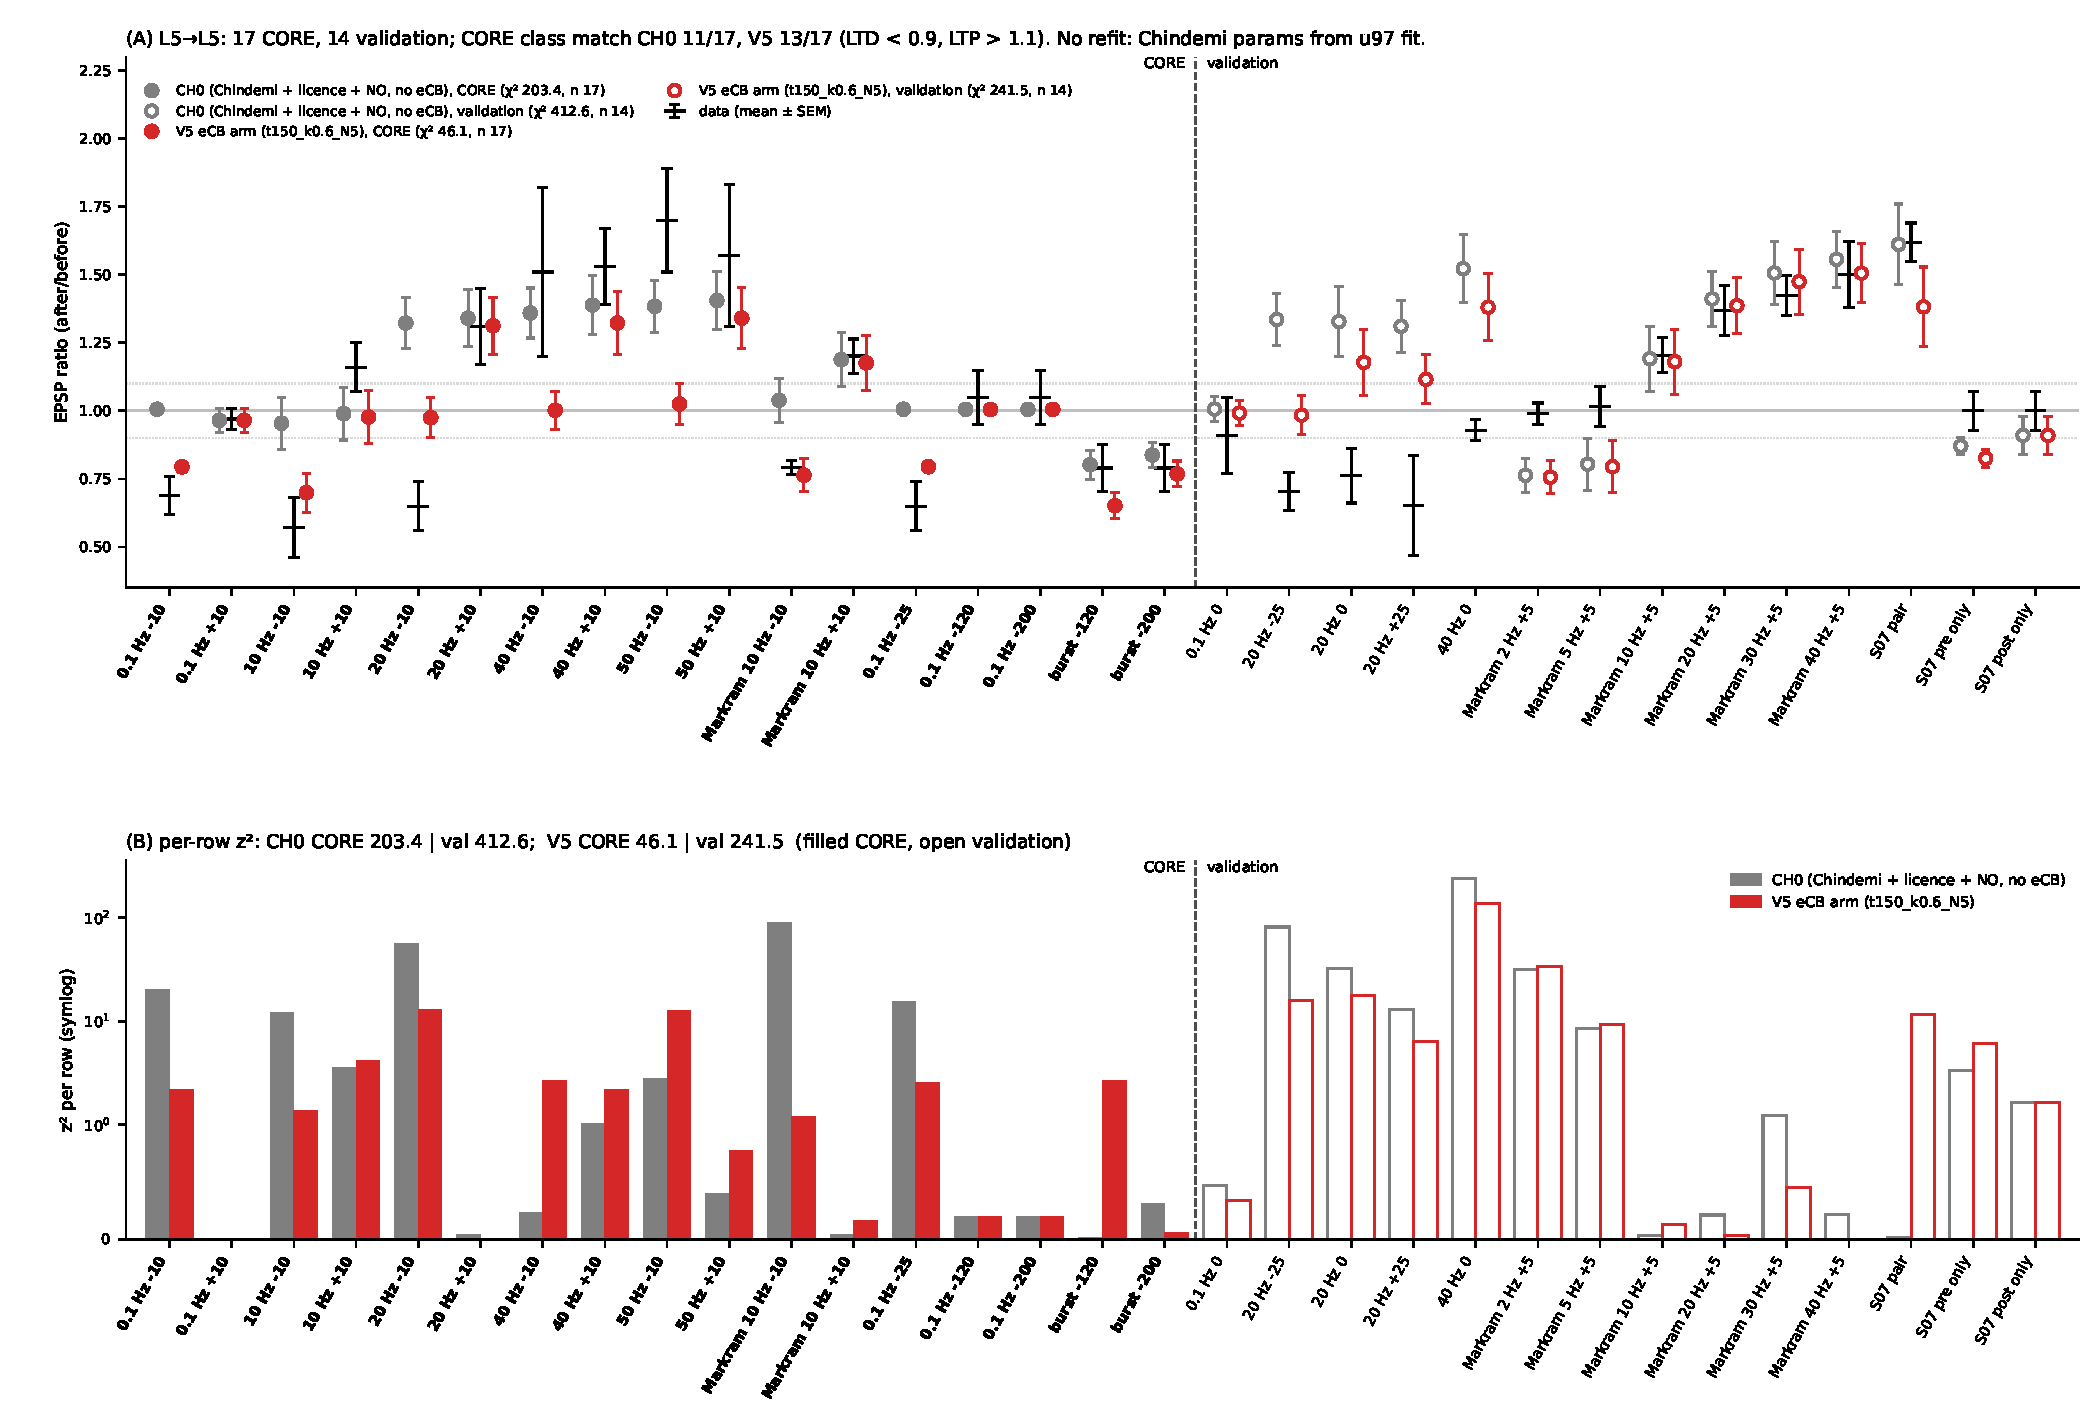
\includegraphics[width=\linewidth]{figV5_vs_CH0.pdf}
\caption{V5 compared with CH0 on L5$\to$L5. (A) EPSP ratio, data mean $\pm$ SEM (black) and model mean $\pm$ SEM over
pairs. Filled points are core rows; open points are validation rows. (B) $z^2$ per row on a symlog axis.}
\label{fig:v5}
\end{figure}

\begin{table}[p]
\centering
\scriptsize
\caption{All L5$\to$L5 rows. Data sources are copied from the target tables. ``Markram 1997'' marks rows whose
target table gives no figure.}
\label{tab:rows}
\begin{tabular}{l l c c c >{\raggedright\arraybackslash}p{6.3cm}}
\toprule
Row & set & data & CH0 & V5 & source \\
\midrule
0.1\,Hz $-10$ & core & $0.69\pm0.07$ & 1.01 & 0.79 & Sj\"ostr\"om, Turrigiano \& Nelson 2001, Fig.~7B (0.1\,Hz bar) \\
0.1\,Hz $+10$ & core & $0.97\pm0.04$ & 0.97 & 0.97 & Sj\"ostr\"om et al.\ 2001, Fig.~1D (0.1\,Hz bar); also Fig.~3B \\
10\,Hz $-10$ & core & $0.57\pm0.11$ & 0.95 & 0.70 & Sj\"ostr\"om et al.\ 2001, Fig.~7B (10\,Hz bar) \\
10\,Hz $+10$ & core & $1.16\pm0.09$ & 0.99 & 0.98 & Sj\"ostr\"om et al.\ 2001, Fig.~1D (10\,Hz bar) \\
20\,Hz $-10$ & core & $0.65\pm0.09$ & 1.32 & 0.97 & Sj\"ostr\"om et al.\ 2001, Fig.~7B (20\,Hz bar) \\
20\,Hz $+10$ & core & $1.31\pm0.14$ & 1.34 & 1.31 & Sj\"ostr\"om et al.\ 2001, Fig.~1D (20\,Hz bar) \\
40\,Hz $-10$ & core & $1.51\pm0.31$ & 1.36 & 1.00 & Sj\"ostr\"om et al.\ 2001, Fig.~7B (40\,Hz bar) \\
40\,Hz $+10$ & core & $1.53\pm0.14$ & 1.39 & 1.32 & Sj\"ostr\"om et al.\ 2001, Fig.~6B legend (153$\pm$14\%, $n=11$) \\
50\,Hz $-10$ & core & $1.70\pm0.19$ & 1.38 & 1.03 & Sj\"ostr\"om et al.\ 2001, Fig.~7B (50\,Hz bar) \\
50\,Hz $+10$ & core & $1.57\pm0.26$ & 1.41 & 1.34 & Sj\"ostr\"om et al.\ 2001, Fig.~1D (50\,Hz bar) \\
Markram 10\,Hz $-10$ & core & $0.79\pm0.03$ & 1.04 & 0.76 & Markram 1997 \\
Markram 10\,Hz $+10$ & core & $1.20\pm0.06$ & 1.19 & 1.18 & Markram 1997 \\
0.1\,Hz $-25$ & core & $0.65\pm0.09$ & 1.01 & 0.79 & Sj\"ostr\"om 2003 Fig.~9C Ctrl $\Delta t=-25$\,ms [digitised] \\
0.1\,Hz $-120$ & core & $1.05\pm0.10$ & 1.01 & 1.01 & Sj\"ostr\"om 2003 Fig.~9C Ctrl $-120/-200/-400$ pooled [digitised] \\
0.1\,Hz $-200$ & core & $1.05\pm0.10$ & 1.01 & 1.01 & as $-120$ (pooled bar) \\
burst $-120$ & core & $0.79\pm0.08$ & 0.80 & 0.65 & Sj\"ostr\"om 2003 Fig.~9C Burst, pre 120 or 200\,ms after [digitised] \\
burst $-200$ & core & $0.79\pm0.08$ & 0.84 & 0.77 & as $-120$ (pooled bar) \\
\midrule
0.1\,Hz 0 & val & $0.91\pm0.14$ & 1.01 & 0.99 & Sj\"ostr\"om 2001 (sjs01\_11) 0.1\,Hz $\Delta t$ 0 [csv] \\
20\,Hz $-25$ & val & $0.70\pm0.07$ & 1.34 & 0.98 & Sj\"ostr\"om 2001 (sjs01\_14) [csv] \\
20\,Hz 0 & val & $0.76\pm0.10$ & 1.33 & 1.18 & Sj\"ostr\"om 2001 (sjs01\_13) [csv] \\
20\,Hz $+25$ & val & $0.65\pm0.18$ & 1.31 & 1.12 & Sj\"ostr\"om 2001 (sjs01\_12) [csv] \\
40\,Hz 0 & val & $0.93\pm0.04$ & 1.52 & 1.38 & Sj\"ostr\"om 2001 (sjs01\_15) pooled 40/50\,Hz [csv] \\
Markram 2\,Hz $+5$ & val & $0.99\pm0.04$ & 0.76 & 0.76 & Markram 1997 (mrk97\_01) [csv] \\
Markram 5\,Hz $+5$ & val & $1.02\pm0.07$ & 0.80 & 0.79 & Markram 1997 (mrk97\_02) [csv] \\
Markram 10\,Hz $+5$ & val & $1.20\pm0.06$ & 1.19 & 1.18 & Markram 1997 \\
Markram 20\,Hz $+5$ & val & $1.37\pm0.09$ & 1.41 & 1.39 & Markram 1997 (mrk97\_04) [csv] \\
Markram 30\,Hz $+5$ & val & $1.42\pm0.07$ & 1.51 & 1.47 & Markram 1997 (mrk97\_05) [csv] \\
Markram 40\,Hz $+5$ & val & $1.50\pm0.12$ & 1.56 & 1.51 & Markram 1997 (mrk97\_06) [csv] \\
S07 paired steps & val & $1.62\pm0.07$ & 1.61 & 1.38 & Sj\"ostr\"om 2007 Results + Fig.~1B (162$\pm$7\%) [text] \\
S07 pre only & val & $1.00\pm0.07$ & 0.87 & 0.83 & Sj\"ostr\"om 2007 Fig.~1B open circles, pooled $n=12$ [digitised; SEM assumed] \\
S07 post only & val & $1.00\pm0.07$ & 0.91 & 0.91 & as pre only (pooled bar) \\
\bottomrule
\end{tabular}
\end{table}

%=====================================================================
\section{What is still wrong}
\begin{itemize}
  \item \textbf{40/50\,Hz, $-10$\,ms.} The data show LTP (1.51, 1.70), but the arm fires there and holds the ratio
        near 1.0. The blank misses about 60\% of these coincidences, because Ca$^{2+}$ is already high at the arrival.
  \item \textbf{20\,Hz, $-10$\,ms.} Already 1.32 under CH0; the arm lowers it only to 0.97, against 0.65 in the data.
  \item \textbf{LTP size at 40/50\,Hz.} $\rho$ caps the LTP at about 1.3--1.4.
  \item \textbf{200\,ms step pairing.} The arm takes it from 1.61 down to 1.38. Its ratio between LTD and LTP is too
        large here.
  \item \textbf{Pre only} gives 0.83 (0.87 already under CH0): a problem of the base model.
\end{itemize}
Most of these misses come from the postsynaptic side. The refit of $a_{00}\dots a_{11}$, $\gamma_d$, $\gamma_p$ with
the arm in place is running. It is seeded from the current best fit and run from two unseeded starts, with the same
targets as before.

%=====================================================================
\section*{References}
\small
\begin{itemize}\setlength{\itemsep}{0pt}
\item Chindemi G, et al.\ (2022) A calcium-based plasticity model for predicting long-term potentiation and depression
      in the neocortex. \emph{Nat Commun} 13:3038.
\item Markram H, L\"ubke J, Frotscher M, Sakmann B (1997) Regulation of synaptic efficacy by coincidence of
      postsynaptic APs and EPSPs. \emph{Science} 275:213--215.
\item Nevian T, Sakmann B (2006) Spine Ca$^{2+}$ signaling in spike-timing-dependent plasticity.
      \emph{J Neurosci} 26:11001--11013. doi:10.1523/JNEUROSCI.1749-06.2006
\item Sj\"ostr\"om PJ, Turrigiano GG, Nelson SB (2001) Rate, timing, and cooperativity jointly determine cortical
      synaptic plasticity. \emph{Neuron} 32:1149--1164. doi:10.1016/s0896-6273(01)00542-6
\item Sj\"ostr\"om PJ, Turrigiano GG, Nelson SB (2003) Neocortical LTD via coincident activation of presynaptic NMDA
      and cannabinoid receptors. \emph{Neuron} 39:641--654. doi:10.1016/S0896-6273(03)00476-8
\item Sj\"ostr\"om PJ, Turrigiano GG, Nelson SB (2004) Endocannabinoid-dependent neocortical layer-5 LTD in the
      absence of postsynaptic spiking. \emph{J Neurophysiol} 92:3338--3343. doi:10.1152/jn.00376.2004
\item Sj\"ostr\"om PJ, Turrigiano GG, Nelson SB (2007) Multiple forms of long-term plasticity at unitary neocortical
      layer 5 synapses. \emph{Neuropharmacology} 52:176--184. doi:10.1016/j.neuropharm.2006.07.021
\end{itemize}

\end{document}
